\documentclass[11pt]{article}

\usepackage[margin=1in]{geometry}
\usepackage{amsmath,amssymb}
\usepackage{graphicx}
\usepackage{booktabs}
\usepackage{microtype}
\usepackage[hidelinks]{hyperref}
\usepackage{natbib}
\usepackage{caption}
\captionsetup{font=small,labelfont=bf}

\title{Network capacity is sometimes compute capacity:\\
an accounting framework and decision boundaries for\\
infrastructure investment in large-scale AI training}
\author{Margaret Nanyonga}
\date{August 2026}

\begin{document}
\maketitle

\begin{abstract}
Operators of large accelerator fleets repeatedly choose between buying more
accelerators and improving the infrastructure around the accelerators they
already own. The metrics in common use do not support that comparison. Model
FLOPs Utilization measures how well a step runs and is blind to failures;
Effective Training Time Ratio measures availability and credits communication
stall as productive work. Neither expresses an infrastructure improvement in
units comparable to an accelerator purchase.

We introduce an accounting framework that assigns every accelerator-second to
exactly one of four terminal fates, productive, blocked, discarded, or
unavailable, and a substitution metric that expresses an infrastructure change
as the number of additional accelerators delivering equal productive throughput.
Calibrating a single compute-side parameter on one published training
configuration, the model predicts a held-out configuration of the same system to
within 1.6\%, and reproduces both Daly's optimal checkpoint interval and a
published closed form for expected training-time ratio.

Three findings follow. First, the gap between availability and useful capacity
is large: at 16{,}384 accelerators our reference configuration reports an
effective-training-time ratio of 0.889 while converting 0.627 of purchased
accelerator-seconds into productive work. Second, the informal practice of
converting avoided idle time directly into an equivalent accelerator count
understates an intervention's value by a factor of 1.4 at 2{,}048 accelerators
rising to 9.9 at 65{,}536, because a marginal accelerator is not fully
productive. Third, no single intervention dominates: across the regimes we
examine, four different interventions rank first, and under parameter
uncertainty at 16{,}384 accelerators additional bandwidth ranks first in 0.6\% of
draws while halving the node failure rate ranks first in 52.3\%. The title's
claim holds in identifiable regimes and fails in others, and we report both.
All results are analytical or simulated; none is a hardware measurement.
\end{abstract}

\section{Introduction}

An operator with a fixed budget can spend it on accelerators or on the
infrastructure that keeps accelerators busy: more fabric bandwidth, a flatter
topology, lower node failure rates, faster fault detection, faster restart,
cheaper checkpoints. The first option is easy to price and easy to justify. The
second is not, because the field lacks a metric that puts the two on the same
axis.

The metrics we do have were built for other purposes. Model FLOPs Utilization
(MFU) relates achieved model FLOPs to peak over the wall-clock of a running
step; a job that loses a third of its life to restarts can still report a high
MFU. Effective Training Time Ratio (ETTR), introduced by
\citet{kokolis2025reliability}, is productive runtime over the job's available
wall-clock; it counts ordinary stepping as productive, so exposed collective
communication is credited as useful work. The two overlap and have different
denominators, so their product is not a capacity fraction.

This paper contributes an accounting framework, a substitution metric, an
attribution rule, and a set of decision boundaries derived from them.

\paragraph{Contributions.}
\begin{enumerate}
\item A four-fate decomposition of accelerator-seconds that is mutually
exclusive and collectively exhaustive by construction, and is asserted
numerically on every model evaluation (Section~\ref{sec:framework}).
\item \emph{Substitution-Equivalent Accelerators} (SEA), which expresses an
infrastructure change as the accelerator count delivering equal productive
throughput, and a measurement of how badly the informal alternative errs
(Sections~\ref{sec:framework} and \ref{sec:results}).
\item An order-independent attribution rule for interacting interventions, with
the finding that recovery improvements are complements rather than substitutes
(Section~\ref{sec:results}).
\item Decision-boundary maps showing which intervention is the strongest
marginal investment in each regime, including the regimes where network
investment is worth nothing and the regimes where no accelerator purchase can
substitute for infrastructure quality at all (Section~\ref{sec:results}).
\end{enumerate}

We do not contribute a new simulator, a new communication model, or a new
reliability model. Each of those exists, and we deliberately reuse standard
formulations so that our predictions can be checked against independent tools
and closed forms.

\section{Motivation and the decision problem}

The immediate motivation is a class of infrastructure argument that is made
qualitatively and decided quantitatively. Vendor material describes pooling
compute across power-constrained campuses, synchronized millisecond traffic
bursts, tail-latency sensitivity, automated hang detection, and high-resolution
telemetry \citep{googlecloud2025network}. Each of these is plausible and none is
accompanied by an independent measurement of how much accelerator capacity it
recovers. We treat that material as motivation only.

The decision problem is concrete. Given a fleet, a workload, and a marginal
budget, which purchase yields the most productive accelerator time? Answering it
requires (i) knowing where accelerator time currently goes, (ii) a common unit,
and (iii) knowing how the answer changes with the operating regime.

\section{Related work}

\paragraph{Simulation and performance modeling.} ASTRA-sim
\citep{won2026astrasim3}, SimAI \citep{simai2025}, and Calculon
\citep{isaev2023calculon} model distributed training performance at fidelities
ranging from closed-form analytical to packet-level. None models failures,
recovery, or checkpointing, and none expresses results as a substitution against
accelerator count. \citet{svedas2025survey} survey this space and catalogue
total-cost models separately from performance simulators, which is itself
evidence that the two are not coupled.

\paragraph{Reliability modeling and measurement.}
\citet{kokolis2025reliability} report eleven months of operation across two
clusters, define ETTR, and give a closed form for its expectation.
\citet{bytedance2025byterobust} report 97\% ETTR on a 9{,}600-GPU three-month
job. AIReSim \citep{pattabiraman2026airesim} simulates failure, recovery,
scheduling, and repair; its authors state explicitly that it models no network
topology, communication time, or bandwidth, and that its parameters are
hypothetical. These works measure or simulate reliability; none prices
reliability against network or accelerator spending.

\paragraph{Network cost.} \citet{wang2023railonly} show that LLM traffic is
sparse enough that removing the spine layer preserves training performance while
cutting network cost by 38--77\%. That is the dual of our question: they
minimize network cost at fixed performance, while we compare marginal network,
reliability, and accelerator spending at fixed budget. \citet{cao2024crux}
demonstrate the mechanism we rely on, that communication contention converts
directly into lost GPU utilization.

\paragraph{Counterfactual accounting.} \citet{lin2025stragglers} use what-if
analysis over a production trace to attribute lost time to stragglers,
establishing the methodological precedent for counterfactual capacity
accounting. Their scope is stragglers within one organization's fleet.

\paragraph{White space.} Reading these together, communication modeling and
failure modeling are each well served but rarely in the same model, cost
comparison appears only at fixed performance, and no inspected work expresses an
improvement as an equivalent accelerator count. We found no prior public work
that combines all four.

\section{Framework and methodology}
\label{sec:framework}

\subsection{Four-fate accounting}

For a pool of $N$ accelerators over a window of $T$ seconds, every one of the
$N T$ accelerator-seconds is assigned exactly one terminal fate: \textbf{productive}
(computation present in the delivered model state), \textbf{blocked} (powered and
allocated but not computing: exposed communication, synchronization wait,
pipeline bubble, checkpoint stall, restart), \textbf{discarded} (computed and then
thrown away: everything between the last durable checkpoint and failure
detection), or \textbf{unavailable} (owned but not usable: down, spare, or stranded).

\begin{equation}
P + B + D + U = N T
\label{eq:identity}
\end{equation}

Two conventions make this exact. Classification is by \emph{terminal fate},
not activity: a second spent computing inside a window later discarded is
discarded, not productive. And re-execution is counted once: after a restart,
the original attempt is discarded and the repeat is ordinary productive and
blocked time. Charging both is the most common error in informal goodput
accounting. Equation~\ref{eq:identity} is asserted on every model evaluation to
a relative tolerance of $10^{-9}$.

The \emph{Useful Capacity Fraction} is $\mathrm{UCF} = P / (N T)$: the share of
what was paid for that became useful work. Its denominator is the pool, so
spares and stranded capacity reduce it.

\subsection{Substitution-Equivalent Accelerators}

Let $\Pi(N, c)$ be productive accelerator-seconds per second for a pool of $N$
under configuration $c$. For a baseline $c_0$ at size $N_0$ and an intervention
yielding $c_1$:
\begin{equation}
\mathrm{SEA}(c_1; c_0, N_0) = \Delta N \quad \text{such that} \quad \Pi(N_0 + \Delta N, c_0) = \Pi(N_0, c_1)
\label{eq:sea}
\end{equation}

SEA prices the alternative correctly, because a purchased accelerator inherits
the fleet's inefficiency rather than arriving fully productive, and it accounts
for the cost of growth, because $\Pi$ is recomputed at the larger size where
communication volume is higher and job mean-time-to-failure is shorter. Where
$\Pi(N, c_0)$ never reaches the target, SEA is unbounded: the improvement cannot
be bought with accelerators at any quantity.

SEA requires no prices. It \emph{is} the break-even cost: an intervention is
worth funding when it costs less than SEA fully-loaded accelerators. This is why
we report no currency figures anywhere in this paper.

The informal alternative, dividing avoided idle and repeated accelerator-seconds
by the measurement window, assumes a marginal accelerator is fully productive.
We compute it alongside SEA so its error can be measured rather than asserted.

\subsection{Attribution}

$\Pi$ is nonlinear in $c$, so SEA is not additive across interventions: relieving
one bottleneck changes what the others are worth. We attribute contributions with
the Shapley value \citep{shapley1953value} over all $2^k$ subsets, which is
affordable because the model is cheap, and we verify the efficiency axiom as a
test.

\subsection{Model}

Compute time follows the standard transformer FLOP accounting
\citep{narayanan2021megatron}. Collective time uses an alpha-beta cost model
applied tier by tier across a scale-up domain, a full-bisection pod, and an
oversubscribed cross-pod layer, with ring costs at each tier. Rank layout is
modeled explicitly, so a data-parallel collective whose members sit one per
scale-up domain does not incorrectly receive scale-up bandwidth. Synchronization
cost uses the Gaussian extreme-value approximation for the maximum of $N$ draws.

Reliability is modeled twice, independently. An analytical path uses renewal
expectations; an event-driven path walks the wall clock, places checkpoints,
draws exponential failure times, and attributes each second as it goes. They
share only the parameter definitions. Agreement between them defines the model's
validity envelope (Section~\ref{sec:validation}).

\section{Validation}
\label{sec:validation}

\subsection{Invariants and closed forms}

Beyond Equation~\ref{eq:identity}, the model satisfies limiting cases
(unbounded bandwidth drives exposed communication to zero; a zero failure rate
drives discarded and restart time to zero; an ideal cluster reaches
$\mathrm{UCF} > 0.999$) and monotonicity in bandwidth, failure rate, and
oversubscription.

Two closed forms derived independently of this model are recovered from it.
Daly's optimal checkpoint interval \citep{daly2006checkpoint} is recovered by
brute-force search over the model's own predicted productive time, within 10\%
at checkpoint costs of 10, 30, and 120 seconds. The expected-ETTR expression of
\citet{kokolis2025reliability} is matched within 5\% at 2{,}048, 8{,}192, and
16{,}384 accelerators in the small-loss regime where that approximation applies.

\subsection{External validation}

We calibrate one compute-side parameter, kernel efficiency, on a single
published anchor and then hold it fixed to predict a different configuration of
the same system \citep{grattafiori2024llama3}. No network or reliability
parameter is tuned at any point.

\begin{table}[t]
\centering
\small
\begin{tabular}{lrrrl}
\toprule
Quantity & Published & Model & Error & Verdict \\
\midrule
Held-out throughput (TFLOP/s per accelerator) & 400 & 406.3 & 1.6\% & pass ($\le$10\%) \\
Held-out BF16 MFU & 41\% & 41.1\% & 0.1\% & pass \\
Interruptions in 54 days & 419 & 526.6 & 25.7\% & pass ($\le$35\%) \\
Job-level ETTR & $>$90\% & 88.8\% & 1.2 pts & pass ($\ge$85\%) \\
Job MTTF at 16{,}384 accelerators & 1.8 h & 1.803 h & 0.2\% & pass \\
Job MTTF at 131{,}072 accelerators & 0.23 h & 0.225 h & 2.2\% & pass \\
\bottomrule
\end{tabular}
\caption{External validation. The held-out configuration doubles data
parallelism at fixed global batch, halving compute per step while spreading the
gradient all-reduce across twice as many pods. Thresholds were fixed before the
comparison ran.}
\label{tab:validation}
\end{table}

The interruption threshold is deliberately loose because the failure rate comes
from a different cluster than the one predicted. The rate implied by the
published interruption count, $3.79 \times 10^{-3}$ per node-day, sits inside the
range reported across the two clusters of \citet{kokolis2025reliability}
($2.34$ to $6.50 \times 10^{-3}$).

\subsection{A validation failure}

The first run failed the ETTR check, predicting 0.600 against a published value
above 0.90. The cause was two misspecified inputs, not the model: the
configuration assumed no replacement capacity, so every failure waited a full
physical repair, and assumed 60-second fully blocking checkpoint writes. Both
contradict the source, which states the cluster held 24{,}000 GPUs while the job
used up to 16{,}000 and that failures were handled by automation. An independent
arithmetic check confirms the diagnosis: at the Daly optimum, combined
checkpoint and lost-work overhead is approximately $\sqrt{2w/M}$, which for a
60-second blocking write and a 2.34-hour MTTF is about 12\%, making an ETTR above
90\% unreachable at this scale regardless of any other parameter. We report the
failure rather than only the corrected result.

\subsection{Validity envelope}

The analytical and event-driven paths agree closely over most of the parameter
space and diverge where mean-time-to-failure approaches recovery time. We define
\emph{recovery pressure} as the share of runtime consumed by discarded work plus
restart. Below 0.25 the two paths agree within 1.4\% on UCF; above it they
diverge to 29.6\% (Figure~\ref{fig:fidelity}). Rows above the threshold are
flagged in the raw output and excluded from headline claims; where such a case
is load-bearing we recompute it with the event-driven path.

\begin{figure}[t]
\centering
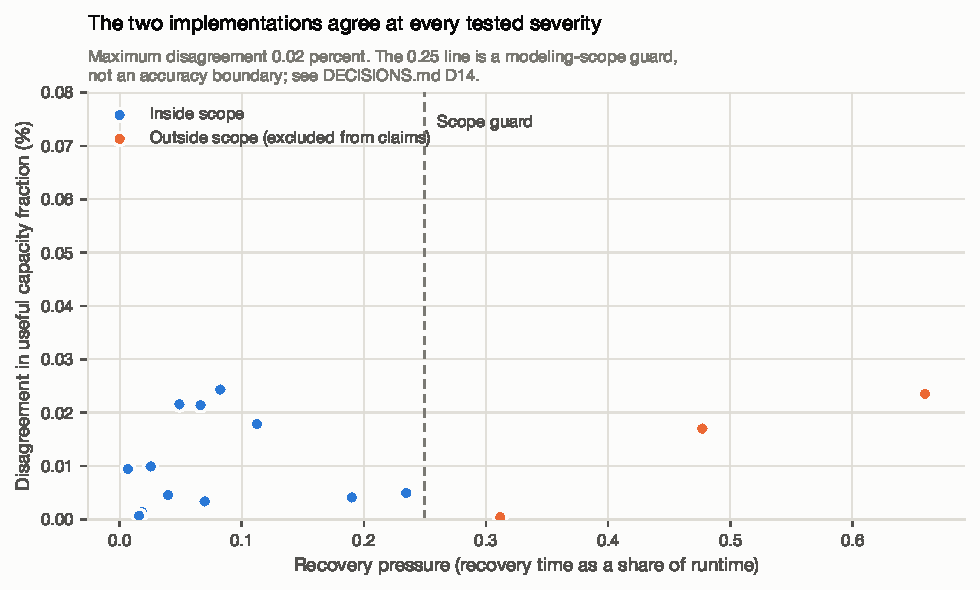
\includegraphics[width=0.62\textwidth]{../figures/fig7_cross_fidelity.pdf}
\caption{Cross-fidelity agreement. The fast path is trusted only where it claims
to be valid, and the threshold is set from this data rather than assumed.}
\label{fig:fidelity}
\end{figure}

\section{Results}
\label{sec:results}

All results below use a study configuration derived from the validated one and
documented separately, so that no study parameter contaminates a validation
claim.

\subsection{Availability is not capacity}

\begin{figure}[t]
\centering
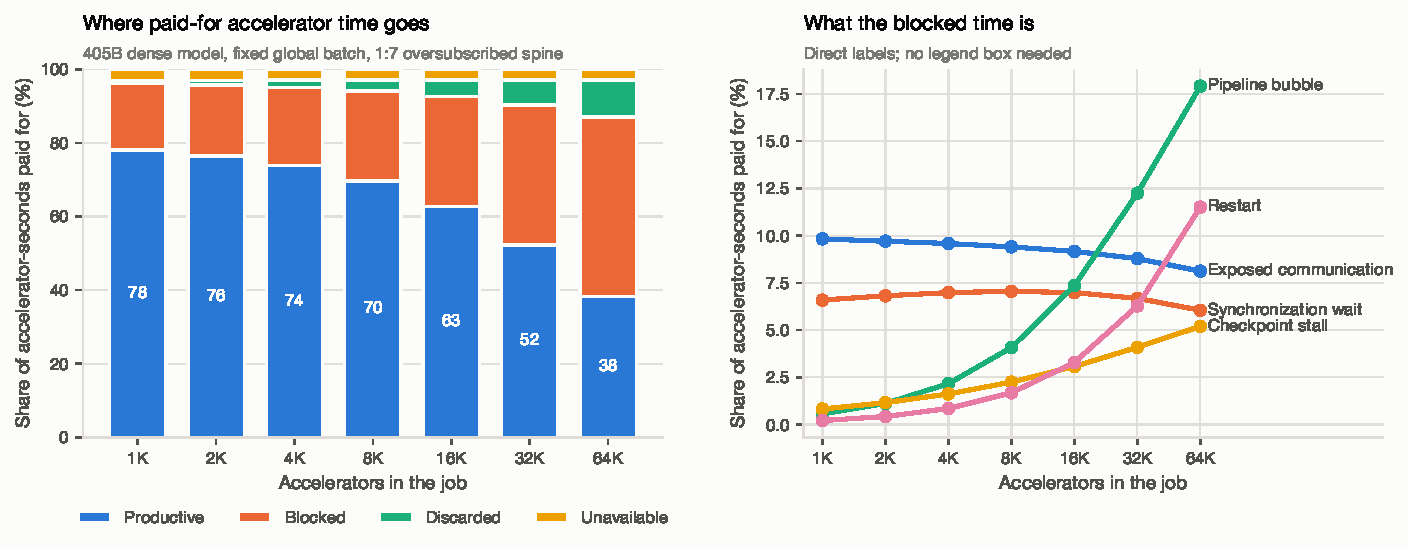
\includegraphics[width=\textwidth]{../figures/fig1_where_time_goes.pdf}
\caption{Where paid-for accelerator time goes as job size grows at fixed global
batch. The productive share falls from 0.781 at 1{,}024 accelerators to 0.382 at
65{,}536. Exposed communication stays near 8--10\% of the total throughout, while
pipeline bubble and restart grow from roughly 1\% combined to roughly 29\%.}
\label{fig:ledger}
\end{figure}

At 16{,}384 accelerators the reference configuration reports
$\mathrm{ETTR} = 0.889$ and $\mathrm{UCF} = 0.627$, a gap of 26.1 percentage
points. An operator reading only ETTR would conclude the fleet is 89\% effective
while 37\% of purchased accelerator-seconds produced nothing. The gap is not a
modeling artifact: it is what ETTR is defined to exclude, namely exposed
communication and the capacity a job never held.

Figure~\ref{fig:ledger} also refines the common framing. Communication is a
roughly constant share of the loss across scale in this configuration; what
grows is pipeline bubble and failure-related time. This is the first place the
paper's title requires qualification.

\subsection{The marginal accelerator}

\begin{figure}[t]
\centering
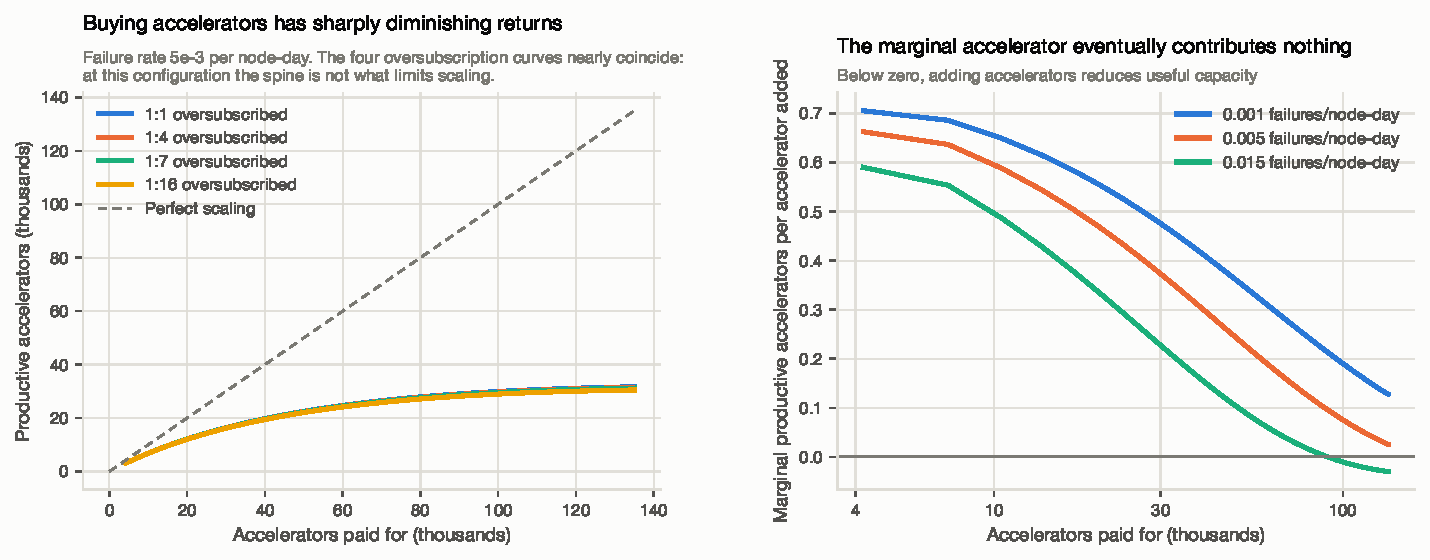
\includegraphics[width=\textwidth]{../figures/fig2_scaling_and_marginal.pdf}
\caption{Productive throughput against pool size, and its derivative. At fixed
global batch the marginal accelerator's contribution falls toward zero and, at
high failure rates, below it.}
\label{fig:scaling}
\end{figure}

At the reference baseline the marginal accelerator contributes 0.444 productive
accelerator-seconds per accelerator-second purchased. This single number drives
the substitution metric: an intervention worth 141 productive accelerators is
worth 318 purchased ones. Notably the four oversubscription curves in
Figure~\ref{fig:scaling} nearly coincide, meaning that at this configuration the
spine is not what limits scaling, a second qualification of the title.

\subsection{The informal metric is biased, and the bias grows}

\begin{figure}[t]
\centering
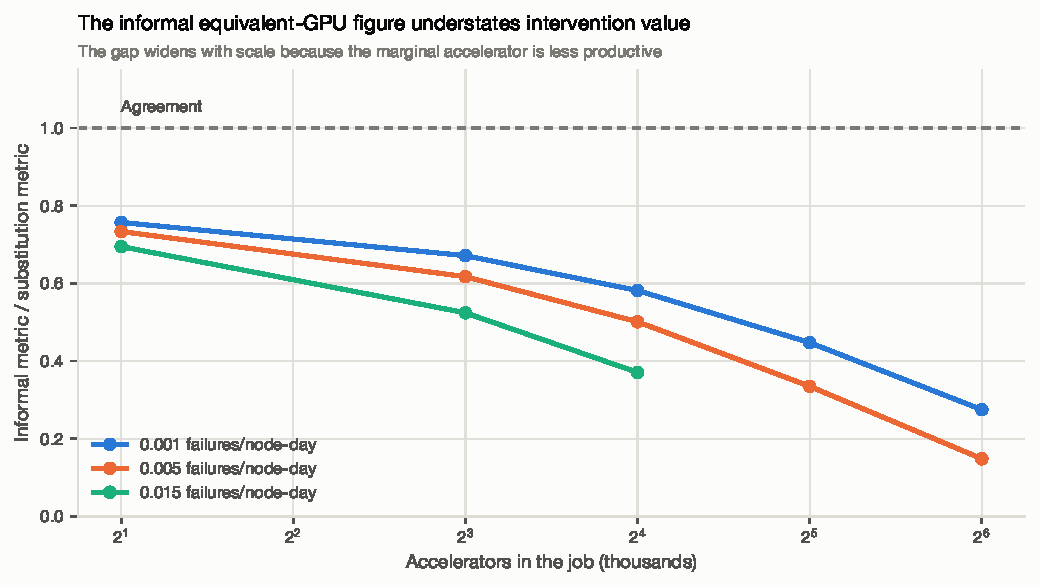
\includegraphics[width=0.68\textwidth]{../figures/fig5_naive_bias.pdf}
\caption{The informal equivalent-accelerator figure as a fraction of the
substitution value.}
\label{fig:bias}
\end{figure}

The informal metric equals 0.72 of SEA at 2{,}048 accelerators and 0.10 at
65{,}536, understating intervention value by factors of 1.4 and 9.9 respectively.
The bias is structural: the informal metric implicitly divides by a marginal
productivity of 1, and the true marginal productivity falls with scale. It errs
most severely exactly where the investment decision is largest.

\subsection{Interventions interact, and not always as substitutes}

Excluding cases where SEA is unbounded, bandwidth and topology improvements are
substitutes as expected (mean additivity error $+6.9\%$), and a mixed network and
reliability bundle likewise ($+10.5\%$). Recovery improvements are
\emph{complements} ($-4.1\%$): faster checkpointing shortens the optimal
checkpoint interval, which shrinks the window of discarded work, which raises
the value of faster detection and restart. This refutes the direction we
hypothesized and is reported as such.

\subsection{Break-even costs}

\begin{figure}[t]
\centering
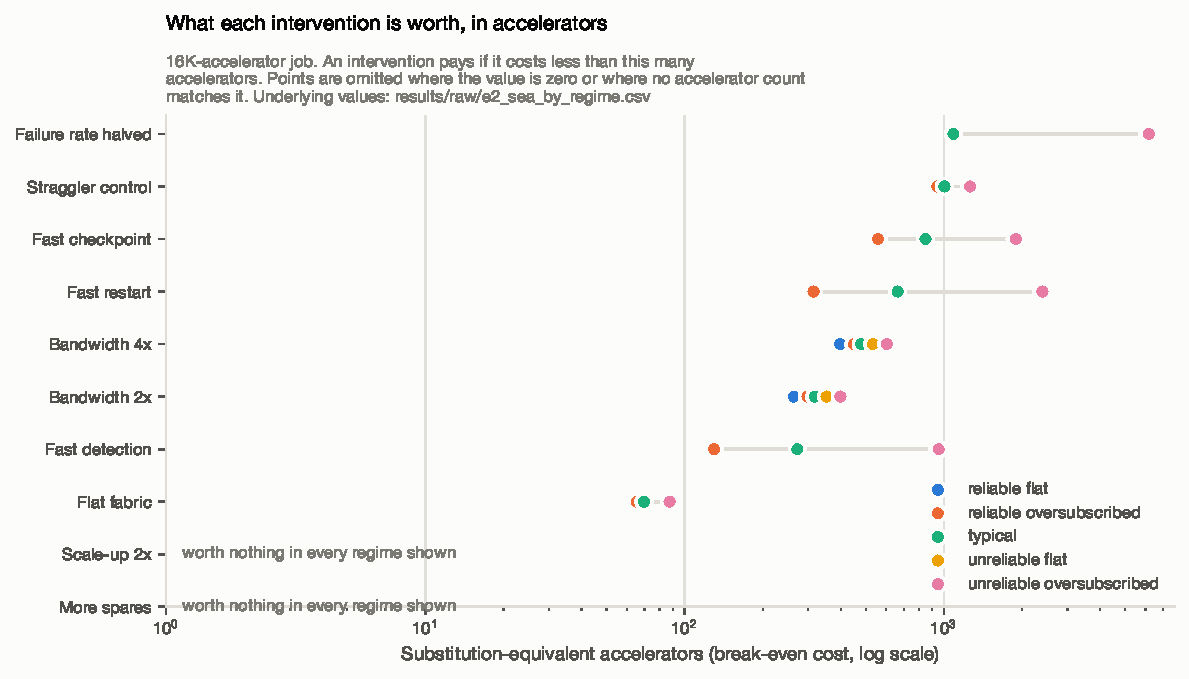
\includegraphics[width=0.82\textwidth]{../figures/fig4_sea_by_regime.pdf}
\caption{Substitution value of each intervention across five regimes at
16{,}384 accelerators, on a logarithmic axis. Because SEA is a break-even cost,
each point states how much an intervention may cost, in fully-loaded
accelerators, before it stops paying. Points are omitted where the value is zero
or where no accelerator count matches the intervention.}
\label{fig:sea}
\end{figure}

Figure~\ref{fig:sea} gives the break-even costs directly. Two features matter
for planning. Enlarging the scale-up domain and adding spares are worth nothing
in every regime shown, because neither relieves a binding constraint at this
configuration. And the spread across regimes is wide: faster restart ranges from
roughly 310 to 2{,}400 accelerators depending on the regime, so a single quoted
value for such an intervention would be misleading.

\subsection{Decision boundaries}

\begin{figure}[t]
\centering
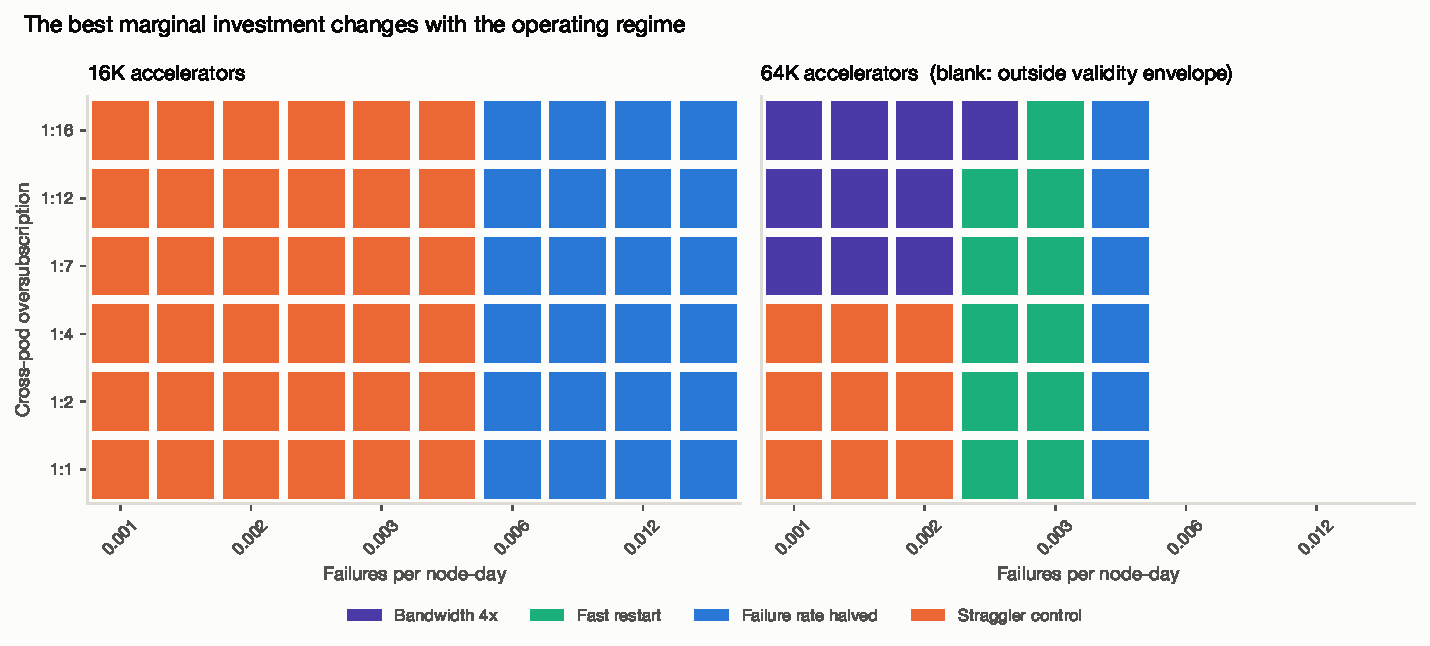
\includegraphics[width=\textwidth]{../figures/fig3_decision_map.pdf}
\caption{The intervention with the highest substitution value, over a
failure-rate by oversubscription grid. Four different interventions rank first,
and the winning set differs between the two scales. Blank cells fall outside the
validity envelope.}
\label{fig:decision}
\end{figure}

Figure~\ref{fig:decision} is the central result. Across 96 in-envelope cells,
four different interventions rank first. At 16{,}384 accelerators the map divides
between straggler control at lower failure rates and halving the failure rate at
higher ones; additional bandwidth never wins. At 65{,}536 accelerators the
picture changes: quadrupled bandwidth wins in the low-failure, heavily
oversubscribed corner, faster restart wins a middle band, and the two
16K-scale winners retain the remainder.

\begin{figure}[t]
\centering
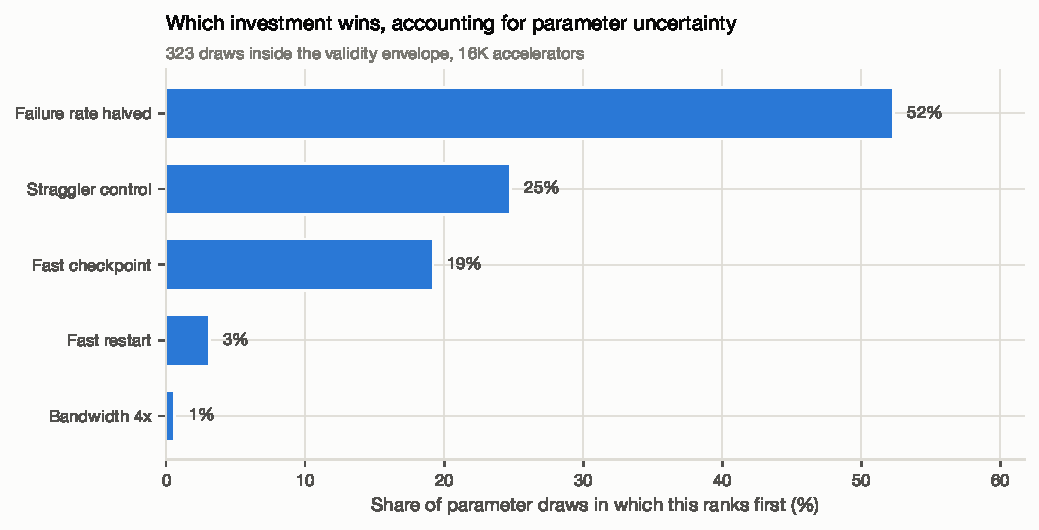
\includegraphics[width=0.68\textwidth]{../figures/fig6_rank_stability.pdf}
\caption{Share of parameter draws in which each intervention ranks first, over
323 in-envelope draws from documented parameter ranges at 16{,}384 accelerators.}
\label{fig:stability}
\end{figure}

Point rankings are not decisions, so we recompute the ranking over draws from
documented parameter ranges (Figure~\ref{fig:stability}). At 16{,}384
accelerators, halving the failure rate ranks first in 52.3\% of draws, straggler
control in 24.8\%, faster checkpointing in 19.2\%, faster restart in 3.1\%, and
quadrupled bandwidth in 0.6\%.

\section{Sensitivity and counterexamples}

We sought negative cases deliberately.

\paragraph{Where network investment is worth nothing.} With an already fast and
flat network (3.2 Tb/s per accelerator, no oversubscription), every bandwidth
and topology intervention has $\mathrm{SEA} = 0$ exactly, while halving the
failure rate is worth 1{,}061 accelerators. The mirror case also holds: with
near-perfect reliability, halving the failure rate is worth zero while doubling
bandwidth is worth 274.

\paragraph{Where nothing much matters.} At 1{,}024 accelerators every
intervention is worth between 2 and 39 accelerators, because $\mathrm{UCF}$ is
already 0.781. Small jobs do not justify infrastructure investment on capacity
grounds.

\paragraph{Where communication dominates.} Shortening the sequence to 2{,}048
tokens or the global batch to 512 sequences raises the value of doubled
bandwidth to 1{,}007 and 1{,}136 accelerators respectively, because
communication becomes a larger share of a smaller step.

\paragraph{Where accelerators cannot substitute at all.} At approximately
131{,}000 accelerators under this configuration, productive throughput
\emph{decreases} as the pool grows: the event-driven path gives 29{,}682
productive accelerators at the baseline pool, 28{,}234 at 1.5$\times$, and
25{,}016 at 2$\times$, while halving the failure rate yields 38{,}075. No purchase
matches the intervention. This case lies outside the fast path's validity
envelope and was confirmed with the event-driven path.

\section{Strategic implications}

The results support three statements an infrastructure planner can act on.

First, measure capacity against what was purchased. A fleet reporting 89\%
effective training time may be converting 63\% of its purchased
accelerator-seconds into useful work, and the difference is where the budget
argument lives.

Second, express improvements as break-even accelerator counts rather than as
recovered time. The conversion is not a formality: the informal version
understates value by up to an order of magnitude at large scale, and it cannot
express the regime where no purchase substitutes.

Third, do not carry a single ranking across regimes. The best marginal
investment at 16{,}384 accelerators with reliable nodes is not the best at
65{,}536 with an oversubscribed spine, and our own thesis fails at the more
common operating points: additional bandwidth ranks first in under 1\% of
uncertainty draws at 16K scale.

\section{Limitations and threats to validity}

\paragraph{No hardware measurement.} Every number here is analytical or
simulated. The external validation compares against published measurements of a
system we did not operate, using a configuration reconstructed from a paper.

\paragraph{The failure process.} Interruptions are modeled as a per-node Poisson
process. This reproduces reported job MTTF at 16{,}384 and 131{,}072
accelerators within a few percent, but misses the measured 1{,}024-GPU MTTF by a
factor of 3.7. The source's own figures are not mutually consistent under
inverse scaling, indicating that small-job interruptions are dominated by causes
we do not model. Results below roughly 4{,}096 accelerators are indicative only.
We also assume failures are independent; correlated failures would worsen
outcomes and would raise the value of fault-isolation interventions we do not
represent.

\paragraph{Scaling policy.} SEA depends on how parallelism is re-planned as the
pool grows. We assume strong scaling at fixed global batch, which is the policy
for finishing a given run sooner. Weak scaling changes the magnitudes, though
not the existence of rank reversals.

\paragraph{Placement.} We assume dense, regular rank placement, the best case for
the network. Fragmented placement would make every network intervention look
better, so this assumption is conservative with respect to our own thesis.

\paragraph{Unvalidated counterfactuals.} No published source reports a system
measured before and after a network or reliability change, so the substitution
metric's inputs are validated but the metric's output is not.

\paragraph{Scope.} Dense transformer pre-training, synchronous, single campus.
No inference, no mixture-of-experts routing, no asynchronous training, no
cross-campus pooling, no absolute costs.

\section{Conclusion}

Network capacity is compute capacity in identifiable regimes, and is not in
others. Deciding which regime a fleet is in requires accounting that closes,
a metric that prices the alternative correctly, and an honest treatment of the
parameters that are not known. We provide all three, along with the cases where
our own thesis fails.

The framework's most useful property may be its least dramatic one: because the
substitution metric is a break-even cost, an operator can apply it without
agreeing with any of our cost assumptions, of which we make none.

\section*{Reproducibility}

The complete implementation, configurations, raw results, and figure scripts are
available at the repository accompanying this paper. The full experiment program
runs in about ten seconds on a laptop and requires no accelerator access.
\texttt{make reproduce} regenerates every number and figure in this paper;
\texttt{make smoke-test} runs a fast subset. Raw results are immutable and carry
provenance sidecars recording the model version, git commit, seed, and
configuration digest. Every threshold in Section~\ref{sec:validation} was fixed
before the corresponding comparison ran.

\bibliographystyle{plainnat}
\bibliography{refs}

\end{document}
